\begin{center}
    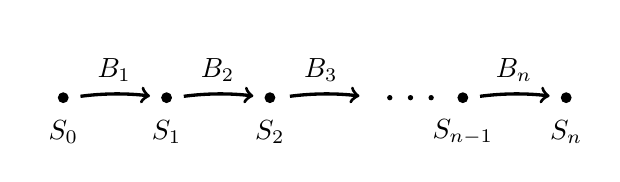
\begin{tikzpicture}[scale=1.75]
        % draw the 0 point
        \draw [thick,color=white] (0,0) -- (0,0);

        % state 0
        \draw [fill=black] (0.25,-0.5) circle (0.035);
        \node at (0.25,-0.75) {$S_0$};

        % block 1
        \draw [very thick, ->] (0.375,-0.49) arc (97.5:83:2);
        \node at (0.62,-0.3) {$B_1$};

        % state 1
        \draw [fill=black] (1,-0.5) circle (0.035);
        \node at (1,-0.75) {$S_1$};

        % block 2
        \draw [very thick, ->] (1.125,-0.49) arc (97.5:83:2);
        \node at (1.37,-0.3) {$B_2$};

        % state 2
        \draw [fill=black] (1.75,-0.5) circle (0.035);
        \node at (1.75,-0.75) {$S_2$};

        % block 3
        \draw [very thick, ->] (1.895,-0.49) arc (97.5:83:2);
        \node at (2.12,-0.3) {$B_3$};

        % ...
        \draw [fill=black] (2.62,-0.5) circle (0.015);
        \draw [fill=black] (2.77,-0.5) circle (0.015);
        \draw [fill=black] (2.92,-0.5) circle (0.015);

        % state n-1
        \draw [fill=black] (3.15,-0.5) circle (0.035);
        \node at (3.15,-0.75) {$S_{n-1}$};

        % block n
        \draw [very thick, ->] (3.275,-0.49) arc (97.5:83:2);
        \node at (3.52,-0.3) {$B_n$};

        % state n
        \draw [fill=black] (3.90,-0.5) circle (0.035);
        \node at (3.90,-0.75) {$S_n$};

    \end{tikzpicture}
    \captionof{figure}{Blocks as transitions between states \label{fig:statemachine}}
\end{center}
